\usetikzlibrary{decorations.markings, arrows.meta} % removed redundant "arrows"

\tikzset{
    midar/.style={
        very thick,
        decoration={
            markings,
            mark=at position 0.55 with {\arrow{latex}}, % Arrow only at the midpoint
        },
        postaction=decorate,
    },
}

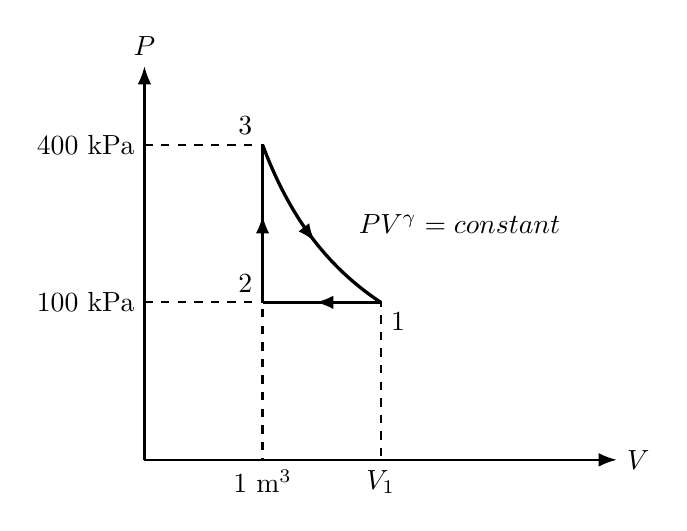
\begin{tikzpicture}[thick]
    % Axes
    \draw[-{Latex}] (0,0) -- (0,5) node[above] {$P$};
    \draw[-{Latex}] (0,0) -- (6,0) node[right] {$V$};

    % Dashed lines for coordinates
    \draw[dashed] (0,4) node[left] {400 kPa} -| (1.5,0) node[below] {1 m$^3$};
    \draw[dashed] (0,2) node[left] {100 kPa} -| (3,0) node[below] {$V_1$};

    % Points and labels
    \node at (1.5,4) [above left] {3};
    \node at (1.5,2) [above left] {2};
    \node at (3,2) [below right] {1};

    % Line segments and hyperbolic curve
    \draw[midar] (1.5,2) -- (1.5,4); % Vertical line from 2 to 3
    \draw[midar] (3,2) -- (1.5,2); % Horizontal line from 1 to 2

    % Hyperbolic curve from 3 to 1
    \draw[midar] plot[domain=1.5:3, samples=100] (\x, {6/\x});
    \node at (4,3) {$PV^\gamma = \text{constant}$}; % Label positioned near the curve

\end{tikzpicture}

